% !TEX encoding = cp1250
\newlength\fwidth
\newlength\fheight

\chapter{Uwagi do wykonywania sprawozda?}
\section{Kodowanie znak?w}
Aktualnie kodowanie znak?w ustawione jest na cp1250 (czasem oznaczane jako windows-1250). Wiele program?w dokonuje automatycznej analizy dokumentu otwieranego i~na podstawie jego zawarto?ci odgaduje jakie kodowanie powinno zosta? zastosowane dla danego pliku. O~ile, przyk?adowo, TeXstudio (dobre IDE na pocz?tek), nie ma problem?w z automatycznym okre?leniem kodowania dla pliku \verb|sprawozdanie_szablon.tex|, poniewa? rozpoznaje np. zawart? w~nim linijk? \verb|\usepackage[cp1250]{inputenc}|, o~tyle pozosta?e pliki tej linijki nie zawieraj?, co powoduje cz?sto b??dnie odgadni?te kodowanie. Aby wskaza? dla danego pliku jakie kodowanie ma zosta? u?yte, mo?na wstawi? na pocz?tku tego pliku linijk? o~tre?ci \newline\verb|% !TEX encoding = cp1250|\newline kt?ra spowoduje wymuszenie u?ycia tego w?a?nie kodowania w~tym pliku.

Oczywi?cie ewentualne przej?cie na kodowanie UTF-8 wymaga? b?dzie:
\begin{itemize}
	\item zmiany linijki \verb|\usepackage[cp1250]{inputenc}| na \verb|\usepackage[utf8]{inputenc}|,
	\item zmiany kodowania w~poszczeg?lnych plikach z kodowania cp1250 na UTF-8,
	\item ewentualn? zmian? linijek \verb|% !TEX encoding = cp1250| na \verb|% !TEX encoding = utf8|.
\end{itemize}
Warto na koniec przekompilowa? wszelkie pliki, aby nie by?o problem?w ze sp?jno?ci?, a~wi?c w~szczeg?lno?ci skasowa? wszystkie pliki o~rozszerzeniu \verb|.aux| i~\verb|.pdf|.

\section{Niemerytoryczne powody niepowodzenia}
Nale?y unika? zrzucania winy za niewykonanie zada? na:
\begin{itemize}
	\item ograniczony czas trwania laboratorium,
	\item b??dy we w?asnym kodzie, kt?rych znalezienie trwa?o zbyt d?ugo,
	\item zbyt du?? liczb? zada? do wykonania,
	\item niedzia?aj?cy sprz?t,
	\item zaskakuj?ce dzia?anie programu, kt?rego nikt si? nie spodziewa?,
	\item itp.
\end{itemize} 

\section{Styl j?zykowy sprawozdania}
Sprawozdanie nale?y pisa? poprawn? polszczyzn?, bez stosowania ?argonu i~anglicyzm?w. Najlepiej stosowa? form? bezosobow?, tzn. sformu?owania typu: zaimplementowano algorytm..., zwi?kszono/zmniejszono parametr..., na rys. ... przedstawiono..., tabela ... przedstawia ... itp.

\section{Zgodno?? z polskimi normami dotycz?cymi przygotowywania publikacji}
Nale?y koniecznie stosowa? klas? \verb+mwrep+ oraz pakiet \verb+polski+. Umo?liwi to przygotowanie dokumentu zgodnie z~normami stosowanymi w~Polsce. Automatycznie zostan? w?wczas regu?y dotycz?ce sk?adu tytu??w, akapit?w itd. Oczywi?cie, nawet zalecana klasa i~pakiet nie zapobiegn? celowym b??dom. Na przyk?ad, nie stosujemy ameryka?skiej formy cudzys?owu, tzn. sekwencji znak?w `` oraz ''.

Nale?y unika? samotnych pojedynczych znak?w (i, a, o, w) na ko?cu wiersza. Aby tego unikn??, stosujemy znak tyldy, kt?ry zabrania przej?cia do nowej linii. Zamiast \verb+w algorytmie+, piszemy \verb+w~algorytmie+.

\section{U?ywanie zwrot?w w~cudzys?owie}
Potrzeba u?ycia wyra?enia otoczonego znakami ,, oraz '', sugeruje, ?e pisz?cy nie zna poprawnego okre?lenia opisywanego zjawiska. W~takim wypadku nale?y zg??bi? k?opotliwy temat lub w~szczeg?lno?ci poprosi? o~pomoc prowadz?cego.

Je?li maj? Pa?stwo jakie? problemy z oprogramowaniem/sprz?tem, to nale?y to zg?osi? prowadz?cemu laboratorium. Nie mniej sprz?t jest testowany przed zaj?ciami -- w~tym aspekcie problem?w by? nie powinno. 

Odwiedzanie prowadz?cego w~ramach konsultacji jest wysoce wskazane i~zalecane. Warto korzysta? tak?e z kontaktu mailowego -- wiele prostych problem?w mo?na rozwi?za? t? drog?.

\section{Separator dziesi?tny}
Stosowanie j?zyka polskiego wymusza na autorze sprawozdania przestrzeganie podstawowych zasad. Jedn? z cz?sto ignorowanych regu? jest stosowanie przecinka zamiast kropki do oddzielenia cz??ci ca?kowitej liczby rzeczywistej od jej cz??ci u?amkowej. Ma to du?y wp?yw na estetyk? sprawozdania. Przecinki stosujemy konsekwentnie na rysunkach, w~tabelach oraz w~tek?cie sprawozdania. Naj?atwiej zadba? o~poprawne stosowanie separator?w dziesi?tnych wykorzystuj?c pakiet \verb+siunitx+ oraz polecenie \verb+\num+. Przyk?ady z?ego i~dobrego zastosowania separatora dziesi?tnego przedstawiono w~tab. \ref{t_przecinki_kropki}.

\begin{table}[H]
	\caption{Przyk?ady z?ego i~dobrego zastosowania separatora dziesi?tnego}
	\label{t_przecinki_kropki}
\centering
\begin{tabular}{llc}
	zapis w \LaTeX & efekt & czy poprawne? \\ \hline
	\verb+$12.345$+ & $12.345$ & nie \\
	\verb+$12,345$+ & $12,345$ & nie \\
	\verb+$\num{12.345}$+ & $\num{12.345}$ & \textbf{tak} \\
	\verb+$\num{12,345}$+ & $\num{12,345}$ & \textbf{tak} \\
\end{tabular}
\end{table}

Nawyk pisania kropek zamiast przecink?w w~liczbach rzeczywistych cz?sto wywodzi si? ze stylu narzuconego przez j?zyk programowania i~dlatego mo?na go zachowa? tylko w~listingach -- w~sprawozdaniu i~na wykresie koniecznie nale?y stosowa? przecinki.

Ciekawe efekty pojawiaj? si? przy wymienianiu r??nych warto?ci parametr?w w jednym zdaniu, np. ,,Do testowania zastosowane zosta?y okresy pr?bkowania $0,01$, $0,1$, $1$, $10$ oraz $100$ sekund.''

\section{Odwo?ania do rysunk?w i~tabel}
Wszystkie rysunki oraz tabele powinny by? ponumerowane oraz by? odpowiednio podpisane. W~tek?cie sprawozdania powo?ujemy si? na rysunki i~tabele podaj?c odpowiednie numery (stosujemy do tego odno?niki, dost?pne w~systemie \LaTeX). Nie stosujemy okre?le? typu: na rysunku poni?ej/powy?ej/3 strony p??niej.

\section{Jednostki}
Przyk?ady z?ego i~dobrego zastosowania jednostek podano w~tab. \ref{t_jednostki}.

\begin{table}[H]
	\caption{Przyk?ady z?ego i~dobrego zapisu jednostek}
	\label{t_jednostki}
\centering
\begin{tabular}{llc}
	zapis w \LaTeX & efekt & czy poprawne? \\ \hline
	\verb+$\num{12.345}\mu s$+ & $\num{12.345}\mu s$ & nie \\
	\verb+$\SI{12.345}{\micro s}$+ & $\SI{12.345}{\micro s}$ & \textbf{tak} \\
	\verb+$\num{12.345}\ \mu s$+ & $\num{12.345}\ \mu s$ & nie \\
\end{tabular}
\end{table}

\section{Wstawianie kodu programu i~jego zasadno??}
Kod programu b?d?cego implementacj? algorytmu wykorzystanego do realizacji zada? laboratoryjnych lub projektowych musi by? dobrze opisany. Opis kodu mo?e by? zawarty w~komentarzach b?d?cych cz??ci? listingu lub zosta? dodany jako osobny fragment tekstu. Podstaw? oceny jest sprawozdanie, w~zwi?zku z czym kod do??czony do sprawozdania w~postaci osobnych plik?w cz?sto nie jest czytany -- jego tre?? s?u?y najcz??ciej do ustalenia samodzielno?ci pracy.

\section{Warunki stosowania \texttt{plot} i~\texttt{stairs}}
Polecenie \verb+plot+ ??czy kolejne punkty odcinkiem, przyk?adowy wykres podano na rys. \ref{r_plot}. Wykorzystuje si? przy prezentacji wynik?w, kt?rych pomiar dokonywany jest w~dyskretnych chwilach, lecz warto?ci sygna?u zmieniaj? si? w~spos?b ci?g?y, a~nie skokowy. Przyk?ad: wykres przebiegu pozycji obiektu w~czasie (og?lnie: wyj?cia procesu).

\begin{figure}[H]
\centering
	\setlength\fwidth{0.5\textwidth}
	\setlength\fheight{0.35\textwidth}
	% This file was created by matlab2tikz.
%
\definecolor{mycolor1}{rgb}{0.00000,0.44700,0.74100}%
%
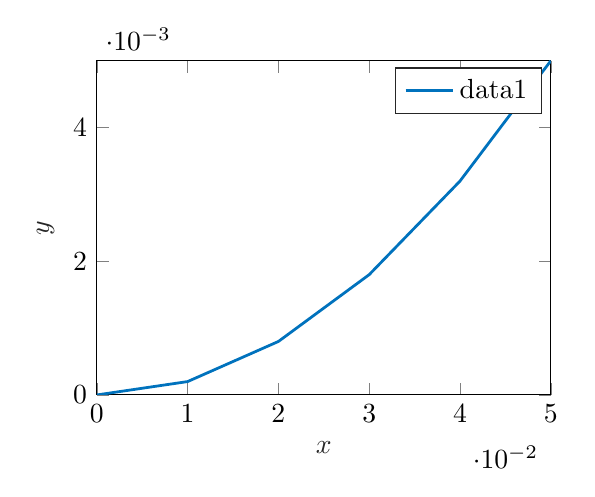
\begin{tikzpicture}

\begin{axis}[%
width=0.951\fwidth,
height=\fheight,
at={(0\fwidth,0\fheight)},
scale only axis,
xmin=0,
xmax=0.05,
xlabel style={font=\color{white!15!black}},
xlabel={$x$},
ymin=0,
ymax=0.005,
ylabel style={font=\color{white!15!black}},
ylabel={$y$},
axis background/.style={fill=white},
legend style={legend cell align=left, align=left, draw=white!15!black}
]
\addplot [color=mycolor1, line width=1.0pt]
  table[row sep=crcr]{%
0	0\\
0.01	0.000199999998666667\\
0.02	0.000799999914666669\\
0.03	0.00179999902800016\\
0.04	0.00319999453866946\\
0.05	0.00499997916669271\\
};
\addlegendentry{data1}

\end{axis}
\end{tikzpicture}%
\caption{Przyk?adowy rysunek uzyskany poleceniem \texttt{plot}}
\label{r_plot}
\end{figure}

Polecenie \verb+stairs+ ??czy kolejne punkty odcinkami r?wnoleg?ymi do osi poziomej, przyk?adowy wykres podano na rys. \ref{r_stairs}. Wykorzystuje si? przy prezentacji wynik?w, kt?rych pomiar dokonywany jest w~dyskretnych chwilach, lecz warto?ci sygna?u zmieniaj? si? w~spos?b skokowy, a~nie ci?g?y. Przyk?ad: wykres sygna?u okresowo zmieniaj?cego si? generowanego przez sterownik programowalny (og?lnie: sygna?y warto?ci zadanych wyj?? oraz sygna?y steruj?ce).

\begin{figure}[H]
\centering
	\setlength\fwidth{0.5\textwidth}
	\setlength\fheight{0.35\textwidth}
	% This file was created by matlab2tikz.
%
\definecolor{mycolor1}{rgb}{0.00000,0.44700,0.74100}%
%
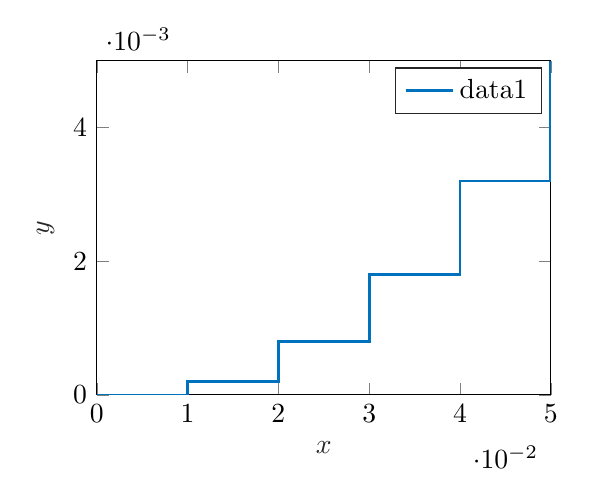
\begin{tikzpicture}

\begin{axis}[%
width=0.951\fwidth,
height=\fheight,
at={(0\fwidth,0\fheight)},
scale only axis,
xmin=0,
xmax=0.05,
xlabel style={font=\color{white!15!black}},
xlabel={$x$},
ymin=0,
ymax=0.005,
ylabel style={font=\color{white!15!black}},
ylabel={$y$},
axis background/.style={fill=white},
legend style={legend cell align=left, align=left, draw=white!15!black}
]
\addplot[const plot, color=mycolor1, line width=1.0pt] table[row sep=crcr] {%
0	0\\
0.01	0.000199999998666667\\
0.02	0.000799999914666669\\
0.03	0.00179999902800016\\
0.04	0.00319999453866946\\
0.05	0.00499997916669271\\
};
\addlegendentry{data1}

\end{axis}
\end{tikzpicture}%
\caption{Przyk?adowy rysunek uzyskany poleceniem \texttt{stairs}}
\label{r_stairs}
\end{figure}

\section{Dodatkowe uwagi dotycz?ce wykres?w}
Umiej?tno?? prezentacji wynik?w rzutuje na to jak sprawozdanie zostanie odebrane i~w szczeg?lno?ci zrozumiane. W~zwi?zku z tym:
\begin{itemize}
	\item aby por?wna? przebiegi czasowe mo?na wy?wietli? wiele przebieg?w na jednym wykresie -- pod warunkiem, ?e dotycz? tego samego sygna?u lub sygna??w por?wnywalnych ze sob? (np. r??ne przebiegi sygna?u wyj?ciowego w~zale?no?ci od zastosowanego parametru),
	\item aby por?wna? przebiegi czasowe mo?na wy?wietli? je jeden nad drugim na r??nych wykresach -- pod warunkiem, ?e skala czasu jest identyczna, a~skala osi pionowej jest r??na na obu wykresach.
\end{itemize}
Kombinacje oraz inne podej?cia s? oczywi?cie r?wnie? dopuszczalne -- nale?y jednak mie? na uwadze, ?e najistotniejsza jest tutaj czytelno??. Czytelnik nie mo?e domy?la? si? intencji autora -- nale?y za?o?y?, ?e zawsze domy?li si? ich niepoprawnie.

Prosz? nie obawia? si?, ?e sprawozdanie b?dzie zbyt d?ugie -- nie s? one drukowane, a~sprawdzaj?cy nie studiuje ka?dego rysunku z osobna. Zamieszczenie nadmiarowych rysunk?w cz?sto jest bardziej op?acalne ni? zaprezentowanie zbyt ma?ej ich liczby -- skutkuje to brakiem istotnych informacji (wykres?w) w~sprawozdaniu. Tak?e je?li wykresy s? do siebie podobne, to warto je zaprezentowa? -- wskazanie skrajnych podobie?stw wykres?w jest cz?sto bardzo istotnym wnioskiem.

\section{Przeprowadzanie eksperyment?w}
Eksperymenty przed ich przeprowadzeniem powinny zosta? zaplanowane. Je?li etap planowania zostanie pomini?ty, mo?e zabrakn?? czasu na realizacj? wszystkich zada? w~ramach laboratorium. Plan eksperymentu powinien tak?e uwzgl?dnia? okre?lenie oczekiwanych rezultat?w lub cel?w, np.:

\paragraph{Przebieg eksperymentu:} Wykonanie pojedynczej skokowej zmiany warto?ci sterowania.
\paragraph{Oczekiwany rezultat:} Pomiary sygna?u wyj?ciowego b?d?ce podstaw? do wyznaczenia odpowiedzi skokowej. Pomiary powinny ustabilizowa? si? po sko?czonej liczbie pomiar?w.

W sprawozdaniu nie ma potrzeby wypisywania eksperyment?w tak jak wy?ej, lecz dla usprawnienia w?asnej pracy warto przygotowa? sobie takie uproszczone opisy.

\section{Krytyczne podej?cie do om?wienia wynik?w}
Podstawowym celem tych zaj?? jest implementacja teoretycznie wspania?ych algorytm?w regulacji do rzeczywistych obiekt?w. Spodziewa? si? wi?c nale?y, ?e teoria nie zawsze b?dzie doskonale pokrywa?a si? z praktyk?. W~takich sytuacjach nale?y wskaza? rozbie?no?? i~wyci?gn?? wnioski z czego ona wynika. Ignorowanie zaskakuj?cych rezultat?w jest niedopuszczalne.

Wszelkie zadania zawieraj?ce s?owo ,,zaimplementuj'' wymagaj? om?wienia implementacji, a~nie zdania ,,Zosta?o zaimplementowane.'' Wszelkie zadania zawieraj?ce s?owo ,,dobierz'' wymagaj? om?wienia sposobu doboru warto?ci ~w szczeg?lno?ci ich oceny pozwalaj?cej na por?wnania ich z pozosta?ymi warto?ciami.

\section{Cykliczna archiwizacja i~analiza wynik?w po laboratorium}
Warto mie? ?wiadomo?? z istnienia w~MATLAB-ie funkcji o~nazwie \verb+save+, kt?ra zapisuje wszystkie istniej?ce w~chwili zapisu zmienne do pliku MATLAB-owego. Pozwala to przede wszystkim na lepsz? organizacj? pracy -- na laboratorium nale?y przeprowadzi? eksperymenty i~zebra? wyniki, a~ich analiz? warto od?o?y? na czas po laboratorium. W~szczeg?lno?ci, warto sprawdzi? czy uzyskane wyniki pokrywaj? si? z rezultatami osi?gni?tymi w~ramach projektu -- oczywi?cie mowa o~zale?no?ciach i~relacjach, a~nie o~dok?adnych warto?ciach.

\section{Om?wienie wynik?w a~dobieranie parametr?w}
Prosz? nie po?wi?ca? przesadnie du?o czasu na poszukiwanie idealnych parametr?w algorytmu regulacji. Pierwszym powodem jest to, ?e takich najcz??ciej nie ma, a~drugim jest fakt, i? nie jest tak bardzo istotna jako?? regulacji osi?gni?ta w~ramach Pa?stwa poszukiwa?, a~raczej zastosowana metodologia i~og?lnie rozumiane podej?cie. Bardziej warto?ciowe jest om?wienie ewentualnych dalszych krok?w maj?cych na celu znalezienie lepszych parametr?w regulacji ni? faktyczne ich poszukiwanie. Prosz? jednak rozs?dnie dobiera? liczb? eksperyment?w, po kt?rej Pa?stwo przerw? poszukiwania -- oczywistym jest, ?e jeden eksperyment to za ma?o, ?eby m?wi? o~jakiejkolwiek tendencji, na podstawie kt?rej mo?naby wyci?ga? wnioski o~dalszych krokach, natomiast 100 eksperyment?w to zdecydowanie za wiele.
